\chapter{Regulator}
\label{cha:regulator}

\section{Zaproponowany regulator}
Do pozycjonowania manipulatora zaproponowany został regulator składający się z dwóch równolegle połączonych regulatorów PID. Kiedy trzymana jest pełna szklanka, to na wyjście przekazywane jest sterowanie z pierwszego regulatora, a kiedy jest pusta to z drugiego. Regulatorom postanowiono zadać inne nastawy, takie, by ograniczyć przyspieszenie kątowe w~sytuacji, gdy trzymana jest pełna szklanka.Ma to na celu spełnienie warunku, by przyspieszenie było małe, aby nie wylać wody. Struktura obu regulatorów jest identyczna, wyrażona następujący wzorem:
\begin{equation}\label{key}
U = (P + I \frac{1}{s} + D\frac{sN}{S+N}) E
\end{equation}
gdzie:\\
$
U$ - sterowanie\\
$E$ - uchyb regulacji\\
$P, I, D$ - współczynniki odpowiednio od części proporcjonalnej, całkującej i różniczkującej.\\
Na podstawie przeprowadzonych symulacji przyjęto następujące nastawy regulatorów:\\
Regulator odpowiedzialny za pozycjonowanie ramienia z napełnioną szklanką:\\
$
P = 7\\
I = 0.2\\\
D = 5\\
$\\
Regulator pozycjonujący ramie z pustą szklanką:\\
$
P = 3\\
I = 0.002\\
D = 1\\
$
Pozycja zadana podawana na regulator manipulatora miała postać funkcji prostokątnej. Stwierdzono jednak, że z uwagi na ograniczenie przyspieszenia, czas pozycji zadanej dla ruchu z pełną szklanką powinien być dłuższy. Na tej podstawie przyjęto czas pozycjonowania ramienia z napełnioną szklanką na 3~s, a czas powrotu ramienia na pozycję początkową na 2~s.\\
Na rysunku \ref{pid_res} przedstawiono odpowiedz układ dla opisanych powyżej regulatorów.
\begin{figure}[h!]
	\centering
	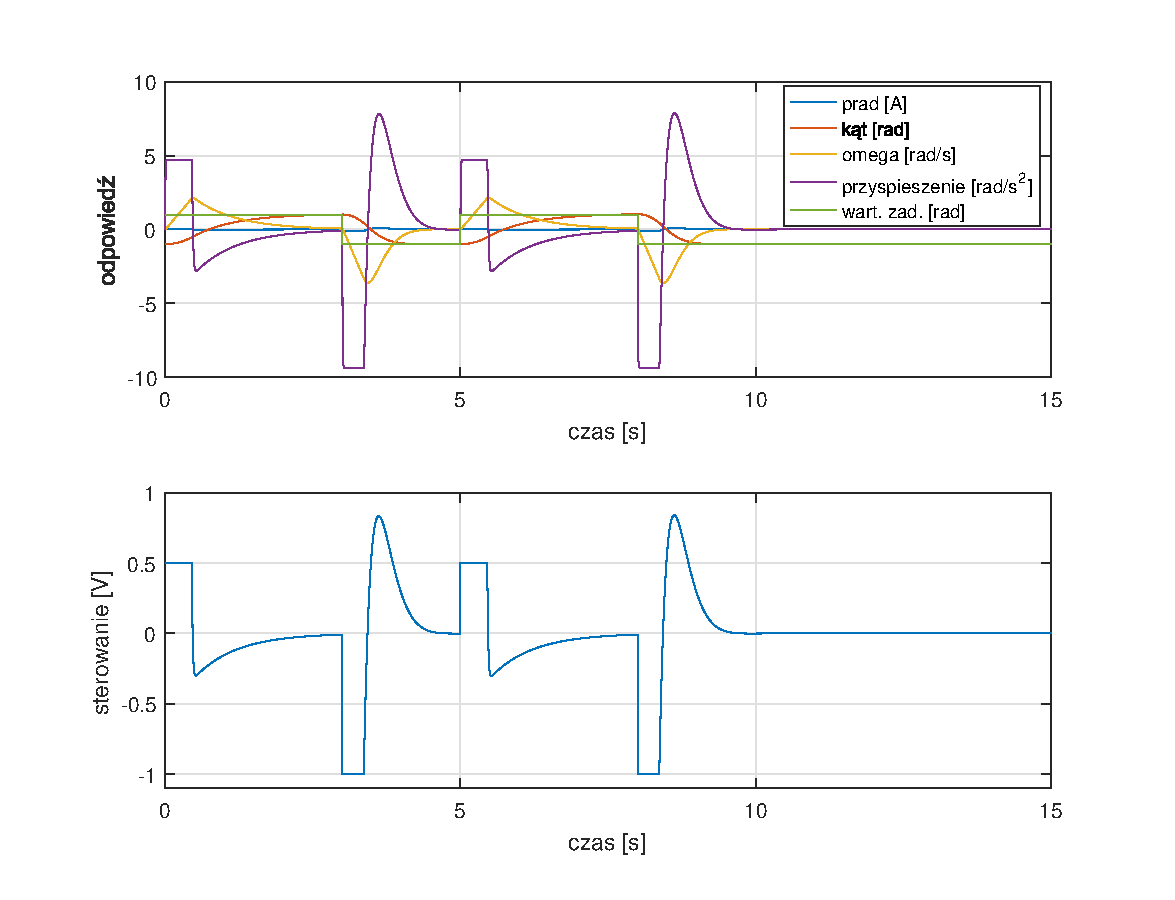
\includegraphics[scale = 1]{fig/pid_response.eps}
	\caption		
	{Wartości zmiennych stanu i sterowania.}
	\label{pid_res}
\end{figure} 
Dla tak przyjętych nastaw regulatorów otrzymano nastepujące wartości wska\'zników jakość:\\
$J_1 = 3.847 \ [rad^2 \cdot s]$\\
$J_2 = 0.7587 [V^2 \cdot s]$\\
$J_3 = 4.606$\\
